\section{Optimal Mechanisms with Both Seller's and Bidder's Cost}

In this section, we take out the constraints and prove that MVAs are optimal in
general. We will also try to find the specific MVA to achieve such optimality,
which turns out to be significantly more complex than previous
simplified case.

The first constraint we are going to remove is seller's cost only.  It is
exciting to introduce bidder's bidding cost since it occurs very often in real
cases and it plays an important role.  Sending emails, making phone calls,
enterring credit card nubmers, depositing money and clicking buttons are all
costly for bidders, though sometimes very tiny.  Bidders may not bid when this
cost is greater than their expected utility. Note that even if the valuation is
very high, the expected utility can be very small because of tense competition,
which is very common on the Internet as $n$, the number of potential bidders,
is very large. 

This behaviour (bidders will not bid because of competitions) is very different
compared to that in previous model \cite{McAfee97:SequentialAuctions} of
sequential auctions. In that model, there is a time discount which
makes bidders eager to bid in early rounds with high reserve prices to avoid
waiting lost. That makes a lot sense in some cases but sometimes it may not.
For example, if the seller posts an auction with a very low reserve price in
the first round, most bidders with high valuation must be happy to bid
according to that time discount cost model. But this may not be true. For
example, when I encounter such an auction online \footnote{For example, when I
see a very good item in the Auction House of Diablo III with a very low current
bidding}, I might be very reluctant to bid because there is a big probability
that my bidding will be over taken by someone else's so it is just a waste of
effort. Our cost model can describe this behaviour very well.

Assume an extreme case where the broadcast cost is $0$, the bidder's bidding
cost is $0.1$ and there are $n \rightarrow \infty$ many $[0, 1)$-uniform
distributed bidders. In a Dutch auction (a Dutch auction has infinite many
rounds of broadcasts so we have to set braodcast cost to $0$), only one bidder
is expected to bid (no competition), thus every bidder with a valuation $v_i
> 0.1$ should be benifitable to bid when the reserve price drops to a little
bit below $v_i-0.1$ (recall that $n \rightarrow \infty$).  In a Vickrey
auction, however, the competition is very tense. Only bidders with valuation
greater than $t$ can accept such intense competition where $t$ satisfies
$t^{n-1}t - 0.1 = 0$ (the expected utility for a bidder with valuation $t$ is
$0$).  Thus $t = \sqrt[n]{0.1}$ which is arbitrary close to $1$ as $n$ grows to
infinity.  Thus almost all bidders cannot bare this competition when $n$ is
really large.

So a bad mechanism (e.g. a Vickrey auction) with too much cost will have less
participations and therefore may decreases seller's profit significantly.  To see
this, look at previous extrame case again.  The revenue of Dutch auction will
converge to $0.9$ (someone with valuation very close to $1$ will bid for price
very close to $0.9$) when $n$ becomes infinity.  The revenue of a Vickrey
auction, however, is only $\int_t^1 x \, (n-1) \,n\,( 1-x) \,{x}^{n-2} dx$
which converges to about $0.67$ when $n$ grows to infinity.  

Another problem caused by bidder's cost is that revenue equivalence theorem
seems to be no longer applicable. That is not strange as the revenue equivalence
theorem assumes that the utility of a bidder is equal to the valuation minus
the payment. This assumption is no longer true as now the utility is also
influenced by the cost charged to this bidder.

Finally, because of allowing bidding costs, it seems that we also have to remove
efficiency constraint. Let us consider the case where the highest valuation is
below the bidding cost. Without compensation to bidders, enforcing efficiency means
bidders with highest valuation have to bid (so we can allocate the item to
them) which would make their expected utility negative.

In summary, we now introduce bidder's bidding cost and drops efficiency
constraint for our mechanisms. The first issue we are going to solve is to make
revenue equivalence theorem, or a very similar theorem, applicable to our model
again. 

\subsection{Spending Equivalence Theorem and Revenue Optimization Strategy}

\begin{theorem}\label{theorem:equivalence}

The expected overall spendings from all bidders (including their bidding costs
and payments to the seller) in a feasible mechanism (with our cost model) is
completely determined by the expected utility of lowest type bidders and
allocation probability function
$$p: (v_1, v_2, \ldots, v_n) \rightarrow (p_1, p_2, \ldots, p_n)$$ 
where $p_i$ is the probability that bidder $i$ will get the item.

\end{theorem}

\begin{proof}
This theorem is exactly the same as revenue equivalence theorem except that we
exchange revenue with spending. To prove it, let us construct another mechanism
$M'$ without bidding cost from our mechanism $M$ with bidding cost so $M'$ fits
into the original revenue equivalence theorem's model. Suppose there is a
virtual seller in $M'$, who collects valuations from all bidders at no cost (a
direct revelation mechanism). Then this virtual seller will make $n$ virtual
bidders delegating bidders to communicate with the true seller in our mechanism
$M$.  When our mechanism ends by allocating the item to virtual bidder $i$, the
virtual seller also allocate the item to the real bidder $i$. The payment from
each bidder $i$ to this virtual seller will be equal to the payment that
virtual bidder $i$ pays to our real seller plus all the bidding costs charged
to virtual bidder $i$. Thus, from the real bidders' aspects, this mechanism
$M'$ is just a direct revelation mechanism which will satisfy revenue
equivalence theorem. The only difference is that the payment from real bidder
$i$ to the virtual seller has two parts, one payed to the real
seller, another consumed by bidding costs.%, which sum up to total spending.
\end{proof}

Thanks to theorem \ref{theorem:equivalence}, our profit maximization problem
is now greatly simplified: 

\begin{corollary}
To maximize profit for a given allocation rule $p: (v_1, v_2, \ldots, v_n)
\rightarrow (p_1, p_2, \ldots, p_n)$, we only need find the minimum total cost
(including both seller's cost and bidders' cost).
\end{corollary}

\begin{proof}
The total spending, substracts cost charged to bidders, will be the revenue
that the seller receives.  This revenue, substracts cost charged to the seller,
will be profit. Thus profit is total spending minus total cost. As total
spending is fixed by allocation rule, we only need to find the minimum cost to
maximze profit.
\end{proof}

The highlight here is that we will not have to differentiate cost charged to
bidders and cost charged to sellers if we just want to maximize seller's profit.
The difference of them may make revenue different, but as long as their sum
does not change, the profit will not change. This not only helps us simplify our
analysis, but also helps us simplify the optimal mechanism: 

\begin{proposition}
In original MVA, to make a set of thresholds $a_i$ works (the
equilibrium holds), we may have to make $r_i$ negative. That says, we need to
compensate bidders if only one bids at reserve price $r_i$ rather than charge
him something, in order to maintain bidders incentive to bid in spite of
bidding cost. That's not intuitive and sellers/bidders may
not be able to easily understand it. A better way to achieve $a_i$ might be
compensating the bidder with the bidding cost immediately after the bidding.
Equivalently, the seller buys the bidding cost for bidders and make it as a
part of seller's bidding cost. This won't change his profit but this will make
everything looks more intuitive ($r_i$ is non-negative again).
\end{proposition}

Now our optimizing problem is greately related to Myerson's if we were able to
minimize the overall cost. However, the optimal allocation rule here is not as
simple as the one that is discovered by Myerson \cite{Myerson:1981}: allocate
the item to the bidder with highest positive virtural value.  Theorem
\ref{theorem:equivalence} tells us that this rule will maximize the total
spending.  But we must substract the cost from the spending to get the profit.
Therefore, there might be another weird allocation rule that has less total
spending but even much less minimum cost.

It is not hard to find one example of this. We know that for bidders
with uniform valuation over $[0, 1)$, the spending maximizing allocation rule
is allocate the item to the bidder with highest valuation that is greater than $1/2$.
However, if the broadcast cost is too large, for example $1$ (which is equal to the
highest possible valuation), the cost to find out whether there is any bidder with valuation
greater than $1/2$ is at least $1$. Thus if we use this allocation rule, the
final profit would be negative since the total spending must be less than the
minimum cost. However, the allocation rule that never allocate the item will have
$0$ cost and $0$ spending, which achieves $0$ profit, better than previous allocation
rule.

Thus, the revenue optimal mechianism will depend on how minimum cost is defined. 
We previously defined how cost is charged and proved that a specific mechanism (MVA)
has minimum cost when allocation rule is allocate efficiently. But unfortunately,
that is not enough to give us a well defined minimum cost for any allocation rule.
For example, one allocation rule might be always allocate the item to each bidder
with the same probability $1/n$, i.e. $p(v_1, v_2, \ldots) = (1/n, 1/n, \ldots)$.
One might think that the minimum cost for this is $0$ since we do not have to know
anyone's valuation. But that cost is not realistic: how can the mechanism ever allocate the
item to someone that it has never communicated with? Thus the minimum cost seems
to be at least $b$, the cost for one round of broadcast, if we ever allocate the item
to some bidder. In order to make a realistic constraint and get a well defined minimum
cost for any allocation rule, we define

\begin{definition}\label{def:allocation_cost}
The allocation rule of a mechanism $$p: (v_1, v_2, \ldots, v_n) \rightarrow
(p_1, p_2, \ldots, p_n)$$ does not allocate blindly if it satisfies: if $p_i >
0$ for some valuation profile $(v_1, v_2, \ldots, v_n)$, there must be a
broadcast query that the $i$-th bidder ($v_i$) reply to the seller
under that profile setting.
\end{definition}

\begin{definition}

Mechanisms satisfy relaxed efficiency constraint with low value $l$
if they always allocate the item to the bidder with highest valuation that's
at least $l$ (no allocation if everyone is below $l$).
%
%    \begin{enumerate}
%
%    \item They only allocate the item to bidders whose valuation are at least
%    $l$ (the low value is $l$)
%
%    \item If they will allocate the item, they will always allocate the item to
%    the bidder with highest valuation.
%
%    \end{enumerate}
%
When we say a mechanism has a low value $l$, we imply that it
satisfies relatex efficiency constraint with low value $l$.

\end{definition}

%With this definition, we have
Then we have

\begin{theorem}
In regular cases (the virtual valuation is monotone strictly increasing~\cite{}),
mechanisms satisfying relaxed efficiency constraint with some low value $l$ are
optimal among all mechanisms that won't allocate blindly.

%The optimal mechanism should always allocate the item to the bidder with
%highest virtual valuation $v_i - \frac{1-F(v_i)}{f(v_i)}$ if it decides to
%allocate the item. In regular cases when the virtual valuation is monotone
%strictly increasing, the optimal mechanism should always allocate the item to
%the bidder with highest valuation if it decides to allocate the item.
\end{theorem}

\begin{proof}
Suppose that there's an arbitrary optimal mechanism. We can describe it by a
query strategy $S(f, m, V, \mathcal Q)$ (see definition \ref{def:query}) and an
allocation function based on $V$, the set of reported values set, since we can
only allocate item to reported bidders. We then construct another mechanism,
with query strategy $S'(f, m, V', \mathcal Q')$ where $\mathcal Q'$ are decsending
and 
\begin{align*}
|S'(f, m, \emptyset, \{Q'_1, \ldots, Q'_{i-1}\})| %= |Q'_i| = |Q_i|\\
  = |S(f, m, \emptyset, \{Q_1, \ldots, Q_{i-1}\})|
\end{align*}
This says, if there's no reported bidders yet, we will always ask the
descending query which has the same length as the query of $S$. And we pretend
that we asked the same query as $S$ so we can continue to ask $S$ what's the
next query length. Once we get reply in $S'$, we terminate the mechanism
immediately and allocate the item to the replied bidder with highest valuation
with probability 1.  Note that we may have $|Q'_i| = |Q_i| = 0$ which means
both mechanisms terminate after $i$ queries without any reply and allocation.
It's clear that our new mechanism won't cause more cost than original
mechanism.  And our new mechanism's allocation rule will get at least as high
total spending as original mechanism because it makes allocation probability of
high value bidders as much as possible. Therefore our new mechanism, which
satisfies relaxed efficiency constraint with some low value $l$, is also
optimal.
%Firstly, note that (at least one) optimal allocation rule $p$ will have at most
%one possible winner, i.e. there can't be $p_i, p_j > 0$ if $i \neq j$. If not,
%without loss of generality let's suppose $v_i \geq v_j$ and $p_i, p_j > 0$. We
%can shift $j$'s probability to $i$, making $p_i' = p_i + p_j$ and $p_j' = 0$.
%Since it can't allocate blindly, this won't increase the cost and actually it
%can potentially lower the cost because we don't need bidder $j$ to reply.  The
%total spending is also non-decreasing by this change in regular cases thus the
%profit is non-decreasing. Keep on doing this change will eventually give us an
%optimal allocation rule with only one possible winner.
%
%Secondly define active region $A$ as
%\begin{align*}
%  A = \{ v_i ~|~ \exists (v_1, \ldots, v_i, \ldots, v_n), p_i > 0 \}
%\end{align*}
%
\end{proof}

For simplicity, we will always assume regularily and will not mention virtual
valuation below.  It's easy to extend our result to general cases by mapping
all values to virtual values and ask broadcast queries according to virtual
values.

\begin{figure*}
\centering
  \subfigure[Best query length $x$ over $h$ with fixed $l$]{
    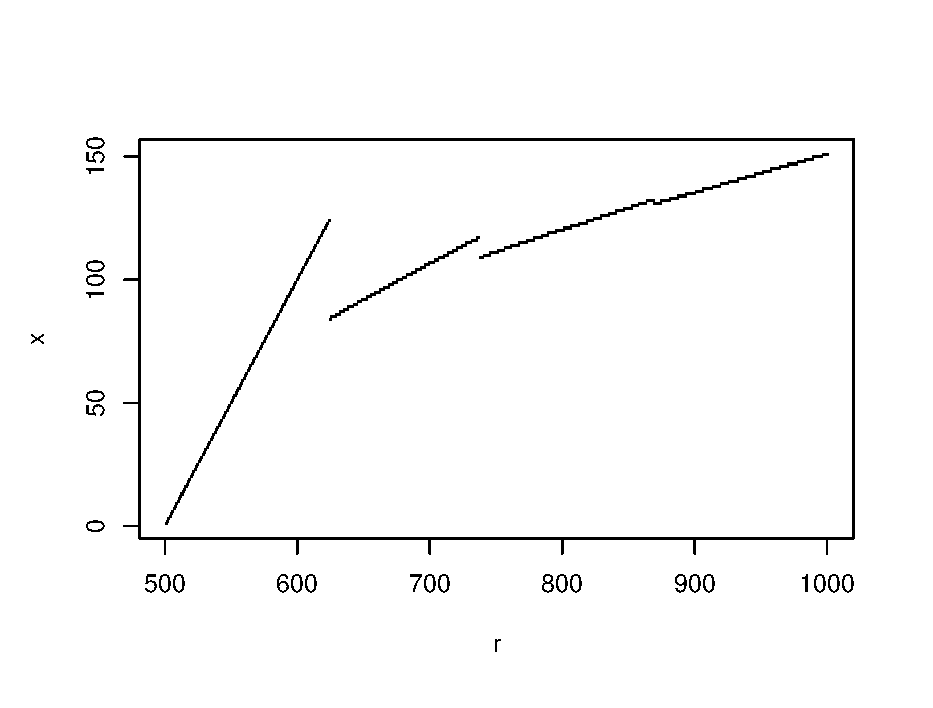
\includegraphics[trim=0mm 5mm 5mm 15mm, clip, width=.4\linewidth]{figures/1000-500-2-1-10}
    \label{fig:x-h}
  }
  \subfigure[Normalized best query length $x$ over low value $l$]{
    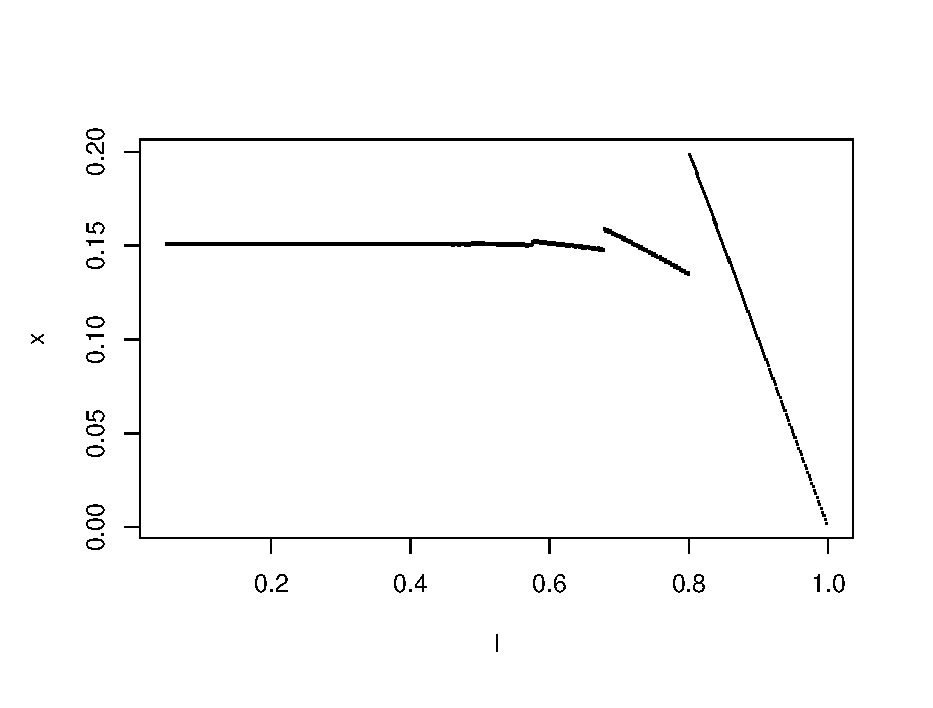
\includegraphics[trim=0mm 5mm 5mm 15mm, clip, width=.4\linewidth]{figures/10000-500-2-1-10}
    \label{fig:x-l}
  }
  \caption{In the first subfigure, we plot the best query length $x = \hat x / D$ over $h = \hat h / D$ (the highest
      undiscovered value) with discretized low value $\hat l = 500$,
      broadcast bidding cost ratio $\rho = 2$,
      number of bidders $n = 10$ and maximum discretized valuation
      $D = 1000$. In the second subfigure, we normalize $x$ to be $x = \hat x / \hat h$ and
      $l$ to be $l = \hat l / \hat h$, as if $h$ is always $1$.}
\end{figure*}

\subsection{MVAs' Optimality in General}

We have already narrowed down optimal mechanism to
relaxed efficient mechanisms and by theorem \ref{theorem:equivalence},
it is straightforward to see

\begin{corollary}

For mechanisms with a fixed low value $l$, the maximum profit is
achieved when the mechanism minizes the cost.

\end{corollary}

Our next question is naturally: what is the cost minimized mechanism
given a low value $l$. 
A similar lemma can be proved using almost identical technique to lemma \ref{lemma:uniform}.
Thus for space limit, we will not elaborate it again. 

\begin{lemma}\label{lemma:lowest_type}
Suppose that there are two cases $n, F_1, f_1, l_1$ and $n, F_2, f_2, l_2$
where $n$ is the number of values for both cases, $F_i, f_i$ are CDF and PDF
of the $n$ i.i.d. values in case $i$, $l_i$ is the low value for case $i$.
If $F_1(l_1) = F_2(l_2)$, then these two cases have the same minimum cost
to find the maximum value above the low value $l_i$.
\end{lemma}

Finally, we conclude

\begin{theorem}

MVAs have the minimum cost among all mechanisms with a low value $l$. Thus
they are optimal.

\end{theorem}

\begin{proof}
A special case of this theorem when $l = 0$ is theorem \ref{theorem:MVA_eq}.
We proved that special case by introducing lemma \ref{lemma:uniform} and
\ref{lemma:descending}. To prove the general cases with arbitrary $l$, we just
need to revise lemma \ref{lemma:uniform} a little to lemma
\ref{lemma:lowest_type}. All other part of the proof remains similar. For space
limit, the detailed proof is omitted.
\end{proof}

Then the only parameters we are going to determine for the
specific optimal MVA are 1) the low value $l$; 2) the descending query
thresholds $a_1, a_2, a_3, \ldots$.
When we later investigate such parameters that minimizes the cost, we will
also assume uniform distribution $F(x) = x$ in default because distribution will not
change this minimum cost and we can always adapt an optimal MVA for uniform distribution
to an optimal MVA for any distribution easily.

\subsection{Experiments to Discover Optimal MVA with a Given Low Value}

To discover the specific MVA that is optimal, we first try to identify the
optimal thresholds $a_i$ given a low value $l$  (recall that in $i$-th round,
MVA will ask all bidders whose valuation is within $[a_i, a_{i-1})$ to bid).
If we can write the minimum cost $C^*$ as a function of $n, \rho, l$ (recall
that $\rho = b/c$ is the ratio between broadcast and bidding cost), we may then
determine the optimal $l$ using this function.

In the special case that we studied in previous section where $l = 0$
(efficiency is enforced), the optimal thresholds can be easily described as a
single parameter $\alpha$. This strategy will not work when $l > 0$ (we assume uniform
distribution in default). Obviously that $a_i \geq l$,
thus we cannot let $a_i = \alpha a_{i-1}$ since $\lim_{i \rightarrow \infty} a_i
= 0 < l$.  Additionally, if we revise the equation by letting $a_i-l = \alpha
(a_{i-1}-l)$, we will get a positive possibility $F(l)$ that we would ask
infinite many broadcast queries, which is even worse.

As it is not immediately clear what optimal thresholds should be like, we
present a simple algorithm to calculate such thresholds numerically. We firstly
discretize the continuous valuation $[0, 1)$ to $D$ discrete values $\{0, 1, \ldots,
D-1\}$. That means, the original valuation $v$ will be transformed to integer
value $\hat v = \lfloor v D \rfloor$. Then we use dynamic programming to
inductively calculate $\hat x_{\hat h}$, the length of next optimal descending
query $[\hat h-\hat x_{\hat h}, \hat h)$ to ask, conditional on that we have
already queried $[\hat h, D)$ and no one replies.

\begin{algorithm}
    \caption{Calculate discretized best query lengths}\label{algo:discrete}
    \begin{algorithmic}[1]
        \Require{$\hat l$ is the discretized low value, $\rho$ is the ratio between broadcast and bidding cost,
        $n$ is the number of bidders, $D$ is the maximum discretized valuation}
        
        \Function{BestQueryLengths}{$\hat l$, $\rho$, $n$, $D$}
            \State $\hat x_{\hat l} \gets 0$
            \State $C_{\hat l} \gets 0$
            \For{$\hat h={\hat l}+1 \mbox{ to } D$}
                \State $\hat x_{\hat h} \gets \displaystyle
                  \operatorname*{arg\,min}_{1 \leq \hat x \leq \hat h-l} \rho + n
                  \frac{\hat x}{\hat h} + (\frac{\hat h-x}{\hat h})^n C_{\hat h-\hat x}$
                \State $C_{\hat h} \gets \rho + n \frac{\hat x_{\hat h}}{\hat h} +
                  (\frac{\hat h-\hat x_{\hat h}}{\hat h})^n C_{\hat h-\hat x_{\hat h}}$
            \EndFor
            \State \Return $\hat x$
        \EndFunction
    \end{algorithmic}
\end{algorithm}

\begin{figure*}
\centering
    \subfigure[$n = 10, b = 0.2, c = 0.1$]{
      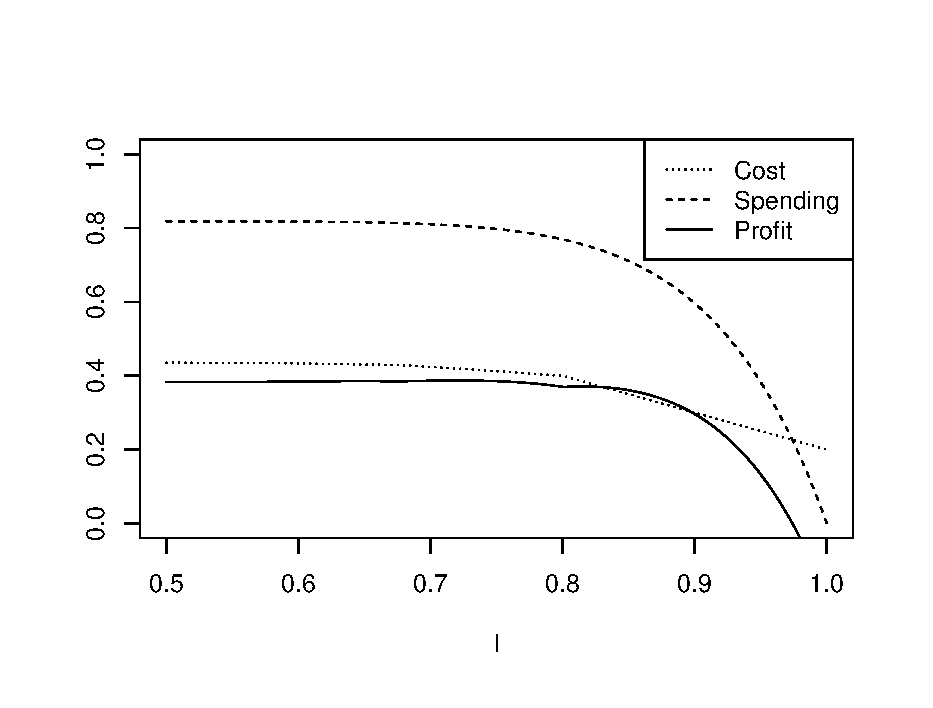
\includegraphics[trim=0mm 5mm 5mm 15mm, clip, width=.32\linewidth]{figures/10-0.200000-0.100000.eps}
      \label{fig:CSP-l-2-1}
    } 
    \subfigure[$n = 10, b = 0.5, c = 0.1$]{
      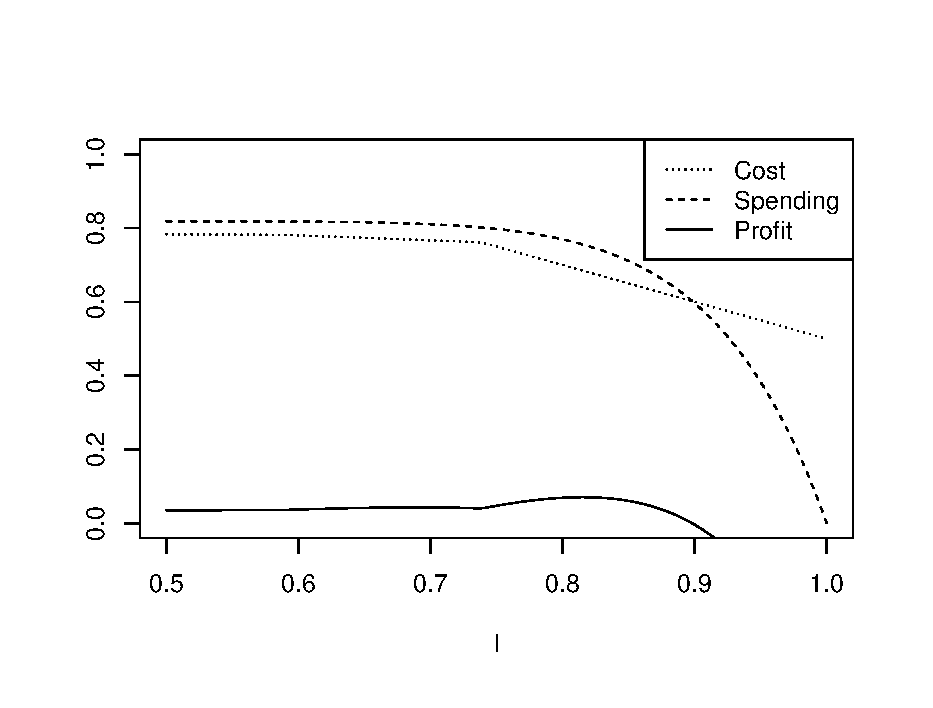
\includegraphics[trim=0mm 5mm 5mm 15mm, clip, width=.32\linewidth]{figures/10-0.500000-0.100000.eps}
      \label{fig:CSP-l-5-1}
    }
    \subfigure[Suboptimality, $n = 10, b = 0.2, c = 0.1$]{
      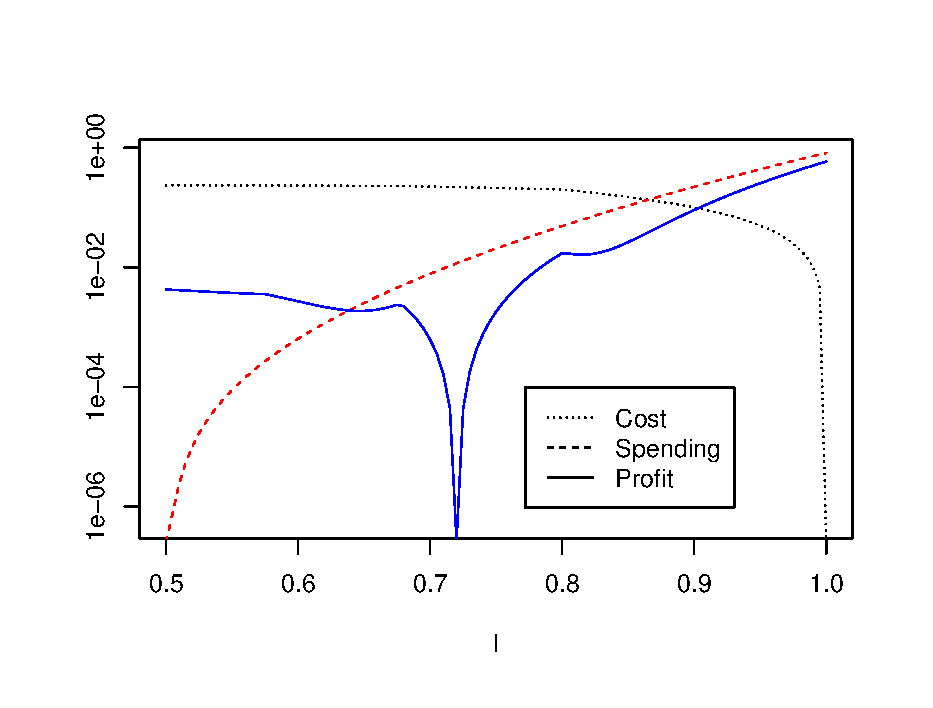
\includegraphics[trim=0mm 5mm 5mm 15mm, clip, width=.32\linewidth]{figures/suboptimality.eps}
      \label{fig:suboptimality}
    }
    \caption{Optimal MVA's cost, spending, profit over $l$, $n$ i.i.d. uniform distributed bidders,
      broadcast $b$ and bidding cost $c$}
\end{figure*}

Algorithm \ref{algo:discrete} runs in time $O(D^2)$. Having $\hat x$, we can
then infer the best strategy $x$ for original continuous problem by converting
$\hat h, \hat x$ back to $h, x$ and using them to interpolate continuous
strategy.  The larger $D$ is the more accurate it will be. But it will also
require more running time.  Running this for case $l = .5, \rho = 2, n = 10, D
= 1000$ we get $x$ showed in figure \ref{fig:x-h}. It seems that $x$ is a
piecewise linear function over $h$.  For those $h$ which is close to
$l$, obviously that the optimal strategy should be $x = h - l$,
which means using only one query to explore all potential bidders. But it is
unclear why $x$ is linear when the best strategy is using multiple queries to
explore the valuation range.

Another way to plot the graph is to normalize $x$ and $l$ so that $h$ becomes
$1$ since our model is $v_i \in [0, 1)$. It is showed in figure \ref{fig:x-l}.
This again looks like a piecewise linear function.  A more interesting
observation is that the left-most piece is quite a long straight line $x =
1-\alpha$. Thus it seems that $x = 1-\alpha$ is optimal for quite a lot $l$ which is not
far from $0$. Here the $\alpha$ is the the optimal $\alpha$ of $\alpha$-MVA if
we set $l = 0$.

\subsection{Analysis of Optimal MVA with a Positive Low Value}\label{sec:general_analysis}

Figure \ref{fig:x-h} shows that the optimal MVA with a low value $l > 0$ is
much more complicated but there might still be hope to get a nice analytical
result: piecewise linear function. That is, we cannot use a single $\alpha$ to
describe such optimal MVA, but perhaps we can use a sequence of $\alpha$ to
describe it. Now let us take an analytical treatment.

The first key to analyze the optimal MVA with $l > 0$ is to utilize
the fact that there is a maximal number of rounds to exploit the whole
reportable valuation range $[l, 1)$. Let us call that
number $k$.\footnote{We have argued this before: if such $k$ does not exist, or equivalently
the maximum number of rounds is unbounded, the cost will be infinite as the possibility that no
values lie in $[l, h)$ is positive.}

For convenience, define $\vec a = (a_0, a_1, a_2, \ldots, a_k)$, the vector of
$k$ thresholds in such optimal MVA. We make $a_0 = h, a_k = l$ so in $i$-th
round the query would be $[a_i, a_{i-1})$. Now define cost $C(\vec a, k, \rho,
n)$ to be the expected cost for MVA defined by $k, \vec a$ when there are $n$
i.i.d.  $[0, 1)$-uniform bidders (note that $l, h$ are implicitly defined by
$a_k, a_0$). If we can get a neat form of $C$, we can use $\frac{\partial
C}{\partial a_i} = 0 $ to characterize optimal MVA, as we did in section
\ref{sec:alpha-MVA}.\footnote{It is easy to see that boundary cases $a_i = a_{i-1},
a_{i+1}$ are not optimal too.}

Thus the second key is to represent this $C$. Rather than
considering one round after another recursively as we did before, we now consider all
rounds together. Let $CR_i$ denote the cost that occur in round $i$ (the broadcast
of that round and the bidding cost charged in that round) and $v^* = \max_i v_i$. Then expected cost
would be sum of expected cost of each round:
\begin{align}
C(\vec a, k, \rho, n) &= \sum_{i=1}^k E[ CR_i ] \nonumber \\
  &= \sum_{i=1}^{k} \Pr\big( v^* < a_{i-1} \big) E[CR_i ~|~ v^* < a_{i-1}] \nonumber \\
  &= \sum_{i=1}^{k} \frac{a_{i-1}^n}{a_0^n} \left( \rho + \frac{a_{i-1}-a_{i}}{a_{i-1}} n \right)
  \label{eq:C_general_simplified}
\end{align}

Taking derivative we get
\begin{align}
 \frac{\partial C}{\partial a_i} = \frac{
	n(n+\rho)a_i^{n-1}-n(n-1)a_{i+1}a_i^{n-2}-n a_{i-1}^{n-1} }{a_0^n}
	\label{eq:diff_C_general}
\end{align}

Unfortunately, equation
\ref{eq:diff_C_general} is not neat enough to get a piecewise linear query length.
Recall that in previous subsection, the experiment seems to show that query length $x$ is
piecewise linear over $h$, which means $a_1 = a_0-x = h-x$ must also be
piecewise linear over $a_0 = h$.  One counter example is the simple case $k = 2, n =
3$. We have: $a_1 =
(\sqrt{{a_0}^{2}\,\rho+{a_2}^{2}+3\,{a_0}^{2}}+a_2)/(\rho+3)$.  Anyway, by
definition we have $a_1 \geq a_2$. And
the former equation indeed looks very linear when $a_1 \geq a_2$.

\begin{figure*}
\centering
  \subfigure[profit]{
    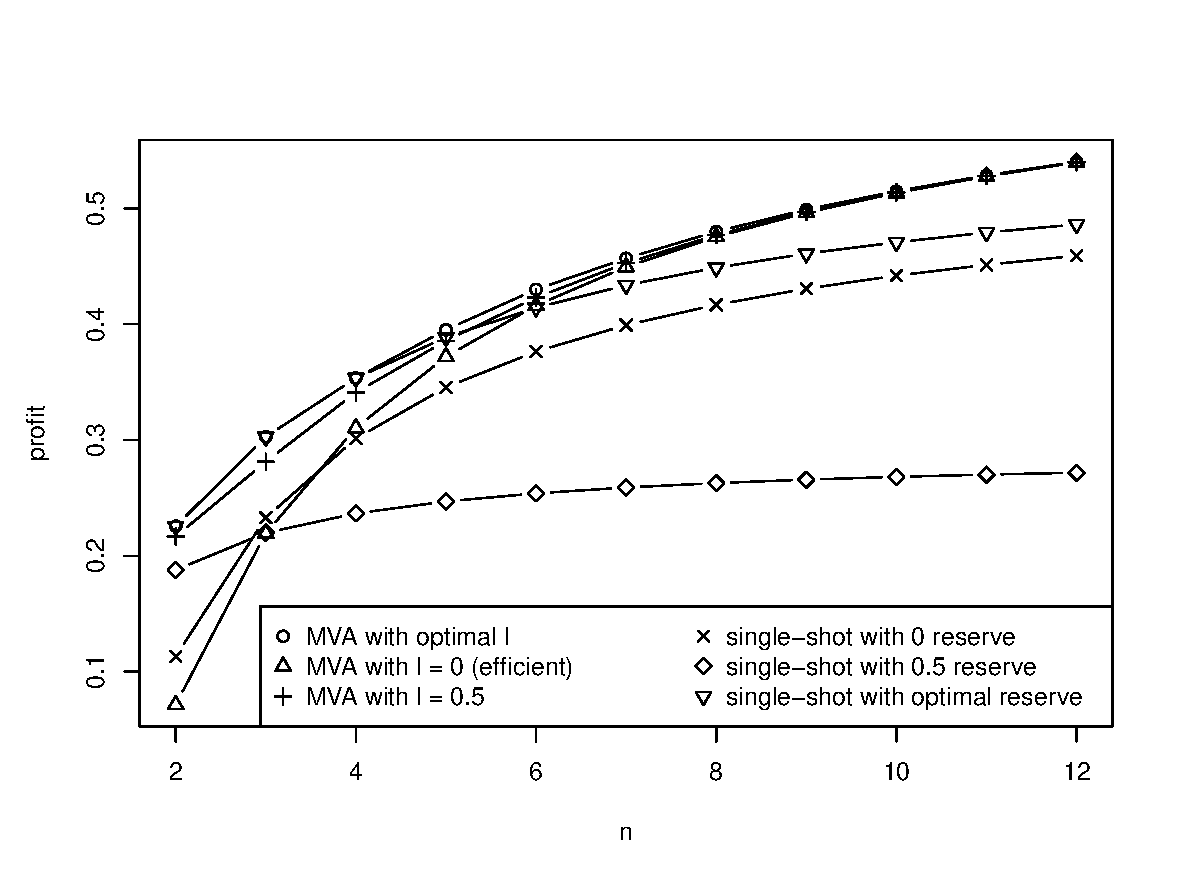
\includegraphics[trim=0mm 5mm 5mm 15mm, clip, height=.3\linewidth, width=.4\linewidth]{figures/profit_.1.eps}
    \label{fig:general_profit}
  }
  \subfigure[low value]{
    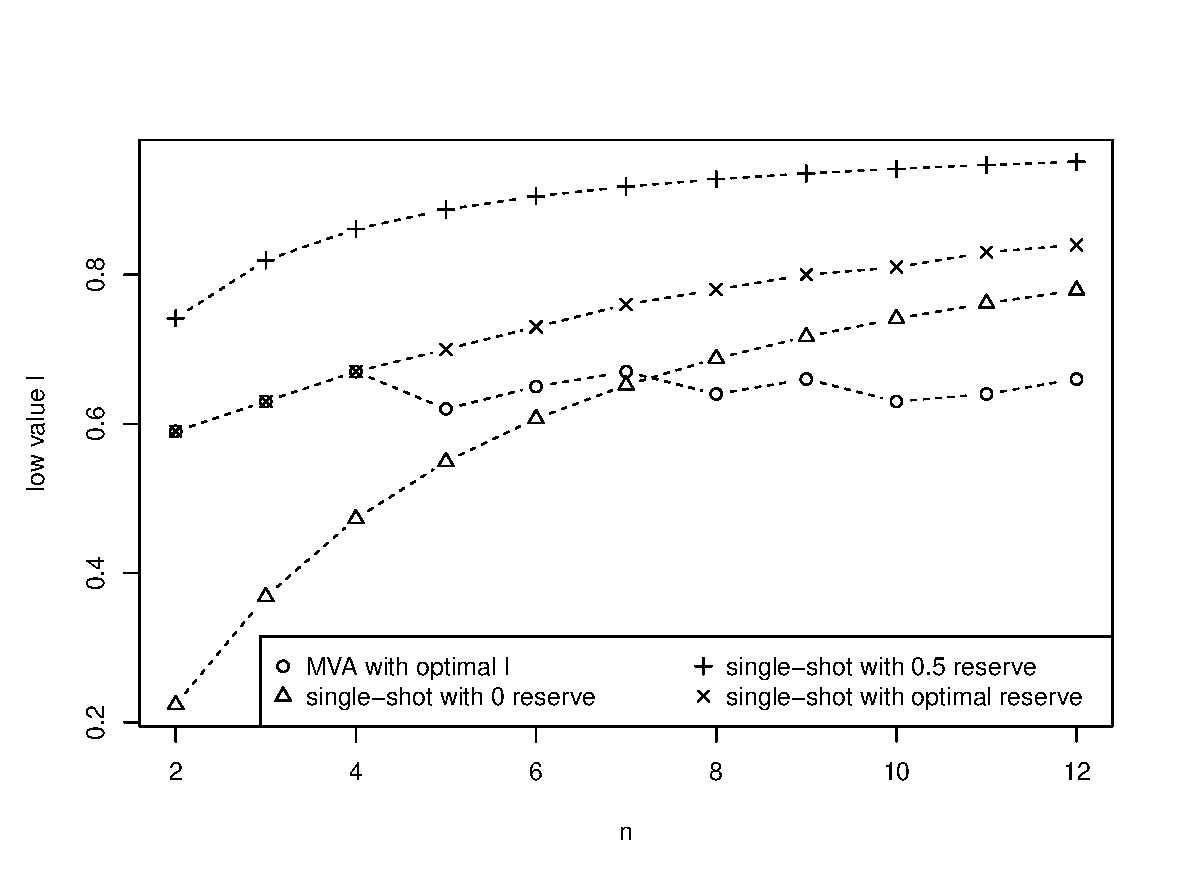
\includegraphics[trim=0mm 5mm 5mm 15mm, clip, height=.3\linewidth, width=.4\linewidth]{figures/l_.1.eps}
    \label{fig:general_l}
  }
  \caption{Compare profit and corresponding low value $l$ over $n$. The
  broadcast cost $b = 0.1$. Bidding cost for seller and buyer are $\beta_1 =
  \beta_2 = 0.05$ (thus $c = \beta_1+\beta_2 = 0.1$)}\label{fig:general}
\end{figure*}

Though we failed characterizing the optimal MVA using piecewise linear
functions, equation \ref{eq:C_general_simplified} gives us a better way to
calculate thresholds $a_i$. We use an R package called BB \cite{Varadhan2009:BB} to
solve these non-linear equation systems. Before throw those equations to that
package, we have to first decide $k$ and an initial guess of $\vec a$.

\begin{lemma}\label{lemma:k_upper}
$k_\alpha = \left\lceil \log_{\alpha} \left(h/l\right) \right\rceil$ is an
upper bound for the optimal $k$. Here $\alpha$ is the optimal $\alpha$ for
$\alpha$-MVA when $l = 0$. 
\end{lemma}

\begin{proof}
We will prove by contradiction. Assume $k > k_\alpha$ for optimal thresholds
$(b_0, b_1, b_2, \ldots, b_k)$ where $b_0 = h, b_k = l$ as defined.  Points
$a_0 = \alpha^0, a_1 = \alpha^1, \ldots, a_{k_\alpha} = \alpha^{k_\alpha}$
split interval $[l, h)$ into $k_\alpha$ subintervals $[a_i, a_{i-1})$, which
together contain $k$ thresholds $b_1, \ldots, b_k$. Since $k > k_\alpha$, at
least one subinterval $[a_i, a_{i-1})$ contain two thresholds $b_j, b_{j-1}$.
Equivalently, there exists $a_i \leq b_j < b_{j-1} < a_{i-1}$.  For
convenience, define $p_2 = a_i \leq q_2 = b_j < q_1 = b_{j-1} < p_1 = a_{i-1}$.

Denote $C(l)$ to be the optimal cost for finding the maximum value above low
value $l$ (suppose $h, n, \rho$ and everything else are constants now). Note
that thresholds $a_0, \ldots, a_i$ must be optimal thresholds for $l = a_i$,
otherwise $\alpha$-MVA can't be optimal.  Similarly, $b_0, b_1, \ldots, b_j$
must be optimal thresholds for $l = b_j$.  Then 
%from optimality of $a_0, \ldots, a_i$ and $b_0, \ldots, b_j$ we have:
\begin{align*}
%  C(b_{j-1}) + b_{j-1}^n [\rho+n(b_{j-1}-b_j)] \leq C(a_{i-1}) + a_{i-1}^n [\rho + n(a_{i-1}-b_j)]\\
%  C(a_{i-1}) + a_{i-1}^n [\rho+n(a_{i-1}-a_i)] \leq C(b_{j-1}) + b_{j-1}^n [\rho + n(b_{j-1}-a_i)]
  C(q_1) + q_1^n [\rho+n(q_1-q_2)] \leq C(p_1) + p_1^n [\rho + n(p_1-q_2)]\\
  C(p_1) + p_1^n [\rho+n(p_1-p_2)] \leq C(q_1) + q_1^n [\rho + n(q_1-p_2)]
\end{align*}
Adding these two inequations together and do some cancellations we get
$p_1^n \leq q_1^n$, which contradicts $q_1 < p_1$.
\end{proof}

The essense of the above proof is the following proposition:

\begin{proposition}\label{prop:thresholds}
Two sets of optimal thresholds can't have $p_2 \leq q_2 < q_1 < p_1$ where
$p_2, p_1$ and $q_2, q_1$ are two consecutive thresholds for these two sets of
thresholds.
\end{proposition}

Having this upper bound, we can eigther bruteforcely search all $k$ between $1$
and $k_\alpha$, or use ternary search [cite wiki?] to get optimal $k$ in
$O(\log k_\alpha)$ time if we can prove it is unimodal.\footnote{We did not
prove that it is unimodal but experiments seems to support this property.}
But in light of the proof above, we actually could have something much better:

\begin{theorem}\label{theorem:k_bounds}
$\left\lceil \log_{\alpha} \left(h/l\right) \right\rceil$ and 
$\left\lfloor \log_{\alpha} \left(h/l\right) \right\rfloor$ are upper
and lower bounds for the optimal $k$. 
\end{theorem}

\begin{proof}
We have already proved the upper bound in lemma \ref{lemma:k_upper}. The
essense of that proof is proposition \ref{prop:thresholds}. If the lower bound
does not hold, we can construct $b_j = p_2 \leq \alpha^i = q_2 < \alpha^{i-1} =
q_1 < b_{j-1} = p_1$, which violates the proposition. 
\end{proof}

By these bounds, we only need to try at most two values to get the optimal $k$.
The next important thing is the initial thresholds $\vec a$. A bad choice may
lead to much more computation and even non-convergence. For example, the
trivial uniform $a_i = (1-i/k)a_0 - (i/k) a_k$ is a bad initial guess. We find
the initial guess $a_i = \alpha^i$ (the same $\alpha$ of $k_\alpha$) to be very
efficient.  Let us call this MVA with thresholds $\alpha, \alpha^1, \ldots,
\alpha^{k-1}$ where $\alpha^{k-1} \geq l, \alpha^k < l$ an $\alpha$-cutoff-MVA,
similar to what we did in previous section \ref{sec:eff_experiment}.  
One explanation about its good performance is that these initial thresholds set
doesn't violate proposition \ref{prop:thresholds}. Thus it's more likely to be
close to actual optimal thresholds set.
%It is
%suggested by experiments showed in figure \ref{fig:x-l} where query length $x$
%seems to be $1-\alpha$ for a lot of $l$. 
In experiments, this $\alpha$-cutoff-MVA's profit is pretty good as shown
in figure \ref{fig:cutoff}. In most cases its profit is very close to optimal.
The significant difference only occur when low value $l$ is a little below
$\alpha$ and this is not likely to occur when $n$ is large where $\alpha$ is
much closer to $1$ than $l$.

\begin{figure}
\centering
    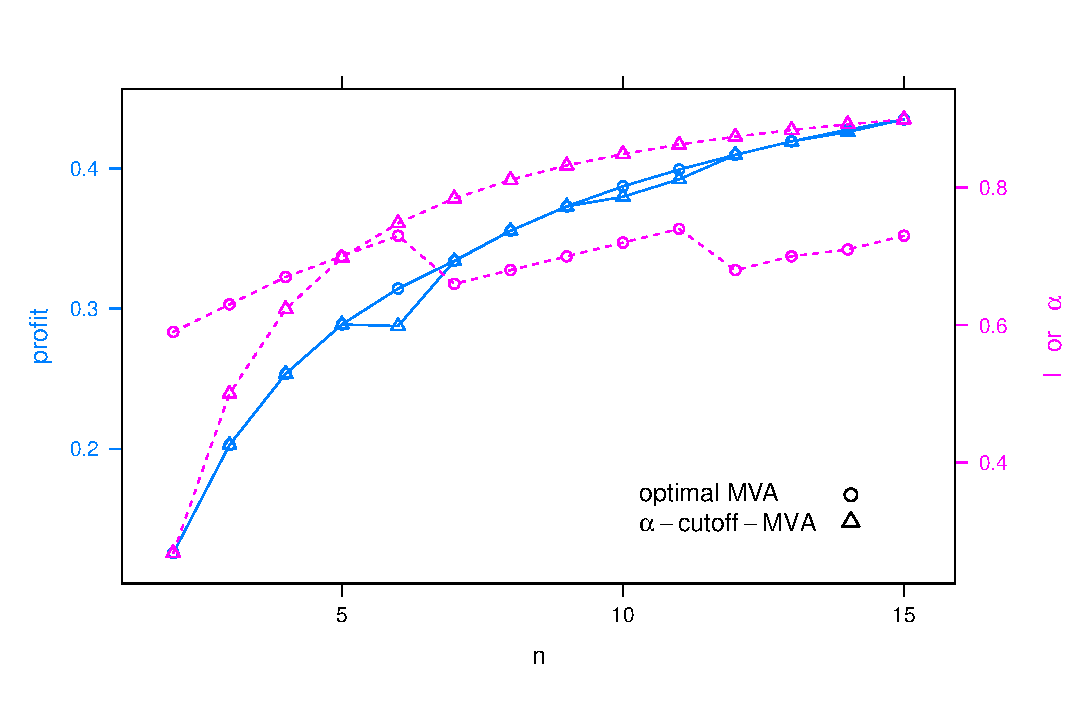
\includegraphics[width=\linewidth]{figures/cutoff_.2_.1_15.eps}
    \caption{The profit of optimal MVA and $\alpha$-cutoff-MVA are plotted in
    solid line.  The low value $l$ is chosen to maximze optimal MVA's profit.
    We also plot $l$ and $\alpha$ in dashed lines to see how they affect the
    relative profit difference.  Note that $\alpha$ does not depend on
    $l$.}\label{fig:cutoff}
\end{figure}

\subsection{Choosing Low Value}

Having $k$ and $a_i$, we are still one step away from optimal MVA: choosing the low
value $l$. It is obvious to see that optimal cost $C$ is non-increasing as $l$
increases. By Myerson's optimal auction theory and theorem
\ref{theorem:equivalence}, setting virtual value of $l$ to be $0$ will yield
the maximum total spending. Name such $l$ as $l_0$. We then conclude that
optimal $l$ must satisfy $l \geq l_0$. The
question is, how to search or determine optimal $l$. Let us first check the simple
case when the value distribution is uniform.

Figure \ref{fig:CSP-l-2-1} and \ref{fig:CSP-l-5-1} plot cost, spending and profit
over $l$. It is clear in figure \ref{fig:CSP-l-5-1} that increasing $l$ from $0.5$ to about $0.8$
will get a significant profit increase. However, it is not so clear in these two plots
whether profit is unimodal and whether we can do ternary search.\footnote{Unlike $k$ which is
an integer with a fairly small upper bound, $l$ is continuous over $[0.5, 1)$, 
thus a ternary search is more needed.}
To see it more clear, we plot figure \ref{fig:suboptimality},
which transforms the cost, spending and profit to their corresponding suboptimality, i.e.
the distance between the specific value and the optimal value (to make the log-scale work
for distance $0$, we add some small constant to that suboptimality). Thus, the new plot will
preserve the peaks and global optimal point as the lowest point.

From figure \ref{fig:suboptimality}, the cost is not unimodal over $l$ and it is quite wierd.
Thus in later experiments, we are just going to brute forcely search over all possible $l$ from $0.5$ to $1$,
with a search increment of $0.01$.

\subsection{Experiments}

Finally we are going to compare profit of different mechanisms in general settings.
To keep it simple, we still use a uniform valuation distribution for all
experiments.  As theorem \ref{theorem:equivalence} shows, the profit is simply
spending minus cost where spending is solely determined by $l$. In fact, the
total spending will not be very sensitive to this $l$ when $n$ is large (except
that $l$ is very close to $1$) and we will see this in later comparisons. Thus
most experimental comparisons that we have done for cost in section
\ref{sec:eff_experiment} would also give us a lot information for profit
comparison. As a result, we will compare mechanisms very different from those
in section \ref{sec:eff_experiment}. Specifically, we will not be interested in
$k$-MVA where $k$ is very limited. Instead, we are going to compare how $l$
is going to affect the profit and how much profit we lose if we ignore the cost.

If we ignore the cost, Myerson has already proved that a singleshot Vickrey
auction with reserve price $0.5$ would be optimal for uniform i.i.d. bidders.
Thus we will compare this singleshot mechanism, as well as its variants, the
singleshot Vickrey auction with $0$ reserve price. But be aware of that reserve
price is not equivalent with low value $l$  when cost exists. To make it more fair,
we add one more singleshot Vickrey auction whose reserve is set to be optimal
among all singleshot Vickrey auctions (i.e. we optimize $l$ for this particular
singleshot mechanism).
One may also suspect whether it is good enough to set low value $l$ to be $0.5$
in such singleshot Vickrey auction, since it will bring us maximal total
spending. The answer is no, because its bidding cost is $0.5 n \times c$, which
grows way too large when $n$ is large.

The experimental result is shown in figure \ref{fig:general}. As shown in
profit comparison figure \ref{fig:general_profit}, the profit of optimal $l$,
$l = 0$ and $l = 0.5$ become close very quickly when $n$ grows and they are
almost identical for $n \geq 8$ in this experiment setting. Thus choosing $l$
will not be a critical issue for large $n$. However, if we use singleshot
mechanism (which is optimal if cost does not exist), the gap is significant.
This is because the bidding cost will drive low value $l$ very
close to $1$ thus lower the total spending significantly. For example, even if
we set reserve price to $0$, when $n = 10$, $l$ will be between $0.6$ to $0.8$.
The optimal reserve price $0.5$ becomes the worst as its $l$ is too high. 
Even if we adapt our reserve price to optimal one, the singleshot mechanism is
still not so good because it cannot balance the total spending and bidding cost,
i.e. it either makes $l$ close to $1$ to lose a lot total spending, or makes
$l$ close to $0.5$ to cause a big bidding cost.
